V celé sekci je zvolena přesnost na 3 desetinná místa. Přesnější hodnoty jsou k nahlédnutí v přiloženém skriptu. Pro zachování přehlednosti nejsou v práci všechny výstupy z Maplu.\\
Zadána byla spodní a horní hranice nepropustného pásma $f_{-s},fs$\,[Hz], spodní a horní hranice propustného pásma $f_{-p},f_p$\,[Hz], maximální útlum v propustném pásmu $a_p$\,[dB] a minimální útlum v~nepropustném pásmu $a_s$\,[dB]. Toleranční schéma definuje oblasti, do kterých nesmí charakteristika filtru zasáhnout. Pro návrh pásmové propusti 4. řádu s Butterworthovou aproximací byly zvoleny parametry tolerančního schématu $f_{-s} = 100$\,kHz, $f_{-p} = 140$\,kHz, $f_p = 160$\,kHz, $f_s = 200$\,kHz, $a_p = 1$\,dB a $a_s = 40$\,dB. Všechny parametry musí být kladná reálná čísla a $f_{-s}$ <  $f_{-p}$ < $f_p$ < $f_s$ a $a_p$ < $a_s$, $f_m$ značí geometrický střed propustného pásma.
\begin{align}
f_{-s} &= \frac{\sqrt{\Delta{fs}^2+4f_m ^2}-\Delta{fs}}{2}\\
f_{-p} &= \frac{\sqrt{\Delta{fp}^2+4f_m ^2}-\Delta{fp}}{2}\\
f_p &= \frac{\sqrt{\Delta{fp}^2+4f_m ^2}+\Delta{fp}}{2}\\
f_s &= \frac{\sqrt{\Delta{fs}^2+4f_m ^2}+\Delta{fs}}{2}
\end{align}
Funkcí $BP2NLP$ byla provedena transformace tolerančního schematu nesymetrické pásmové propusti (PP) na toleranční schema normované dolní propusti (NDP). Byl spočítán nový kmitočet pro horní hranici nepropustného pásma $f_s = 112$\,kHz, geometrický střed propustného pásma $f_m = 149.666$\,kHz, šířka propustného pásma $\Delta{f_p} = 20$\,kHz a šířka nepropustného pásma $\Delta{f_s} = 88$\,kHz. Byl obdržen kmitočet hranice nepropustného pásma normované dolní propusti (NDP) $Os = 4.4$\,1/s.
\begin{figure}[h]
\centering
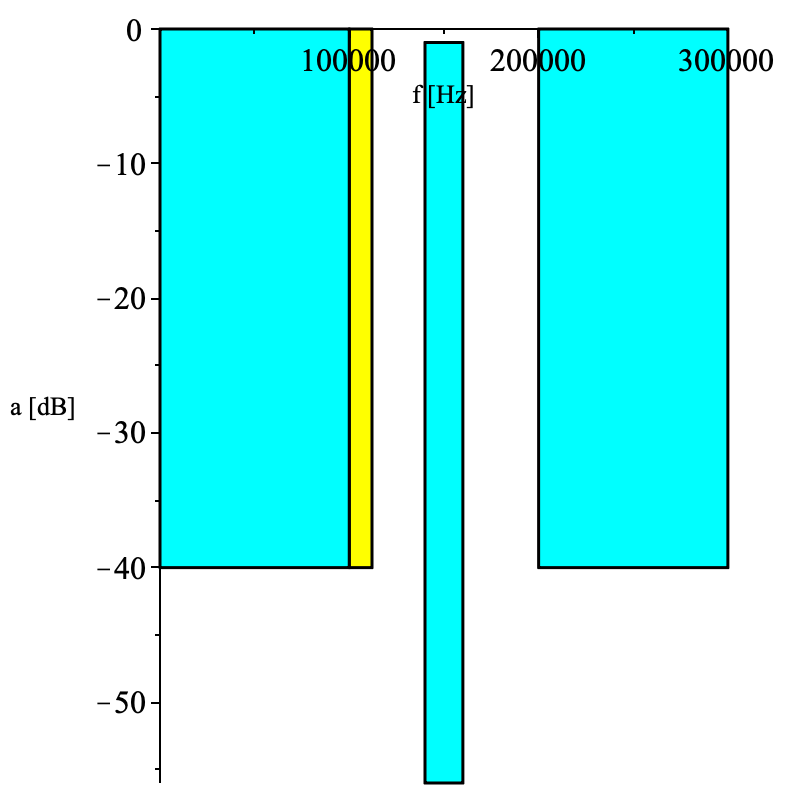
\includegraphics[scale=0.45]{maple1.png}
\caption{Toleranční schéma navrhované pásmové propusti}
\end{figure}
\noindent Stupeň Butterworthovy aproximace normované dolní propusti byl určen jako $order = 4$.
\noindent Dále byla funkcí $Butterworth\_asnew$ určena nová hodnota útlumu v~nepropustném pásmu NDP $a_{snew} = 45.608$\,dB.\\
\\
Následně byl pomocí funkce $Butterworth$ spočten provozní činitel přenosu $G$ jako racionální lomená funkce $G(p) = 1/H(p)$, charakteristická funkce $Phi$ jako $\Phi(p)$ s nulami a póly na imaginární ose. Charakteristická funkce má shodný jmenovatel s $G(p)$. Vypočten byl koeficient nejvyšší mocniny polynomu ve jmenovateli přenosové funkce $Gc = 0.509$, póly $P$ přenosové funkce pomocí funkce $ButterworthPoles$. Počet pólů je dán řádem filtru $order$.
\begin{equation}
P = 
\begin{bmatrix}
-1.094 + 0.453I & -1.094 - 0.453I & -0.453 + 1.094I & -0.453 - 1.094I
\end{bmatrix}
\end{equation}
\begin{align}
G &= 0.509s^4 + 1.574s^3 + 2.435s^2 + 2.207s + 1\\
Phi &=  0.509s^4
\end{align}
\begin{figure}[h]
\centering
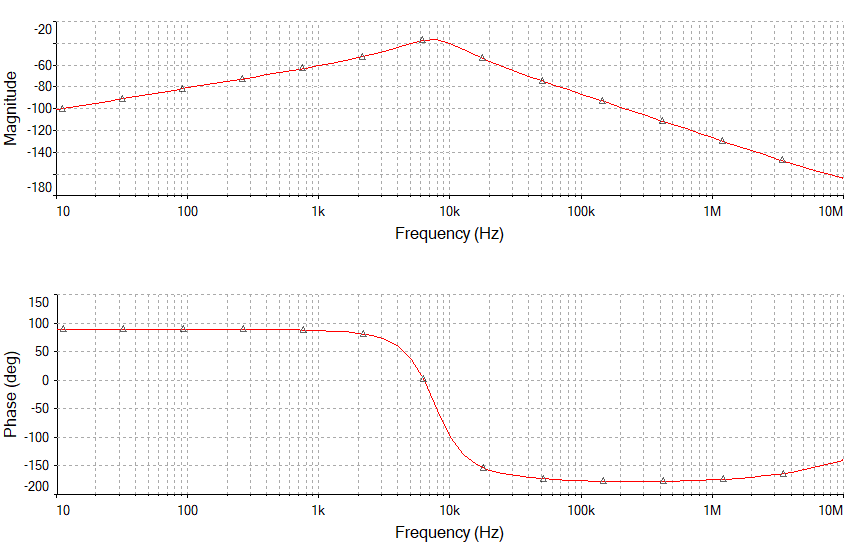
\includegraphics[scale=0.45]{maple2.png}
\caption{Modulová frekvenční charakteristika NDP}
\end{figure}
\noindent Charakteristika byla vykreslena z přenosu funkcí $MagnitudeHdB$, která vypočte modul přenosu podle předpisu |H(j$\omega)$| a výsledek převede na $20 \cdot log_{10} |H(p)|$.
\subsection{Výpočet prvků LC filtru a přenosových funkcí}\label{s:VYP}
\noindent Funkcí $DroppNLP$ byly vypočteny prvky LC příčkového filtru typu normovaná dolní propust (NDP). Zakončení bylo zvoleno standardní (\textit{common}), odpory o hodnotě 1\,$\Omega$, směr zpracování od posledního prvku (\textit{rear}), s T strukturou (začíná zepředu podélným induktorem). Standardní (\textit{common}) zakončení je oboustranné ($R_1~\neq~0, R_z~\neq~\infty$). Výstupem funkce je LC struktura s orientací prvků ve větvi podélně (\textit{direct}) nebo příčně (\textit{shunt}).
\MapleOutput{block (1), [orientation = direct, elements = {L1 = 0.646}, Z = p L1]}
\MapleOutput{block (2), [orientation = shunt, elements = {C1 = 1.561}, Z = \frac{1}{pC1}]}
\MapleOutput{block (3), [orientation = direct, elements = {L1 = 1.561}, Z = p L1}
\MapleOutput{block (4), [orientation = shunt, elements = {C1 = 0.646}, Z = \frac{1}{pC1}]}
\noindent Přenosová funkce pasivních a aktivních struktur filtru byla spočtena funkcí $MakeH$. Byl spočten  napěťový i~výkonový přenos.
\begin{align}
H_{NLPV} &= \frac{1}{1.018p^4  + 3.149p^3  + 4.871p^2  + 4.414p + 2}\\
H_{NLP} &= \frac{1}{0.509p^4 + 1.574p^3 + 2.435p^2 + 2.207p + 1}
\end{align}
\noindent Z rozložení pólů je patrné, že obě přenosové funkce jsou stabilní.
\begin{align}
1.018p^4  + 3.149p^3  + 4.871p^2  + 4.414p + 2 &= 0 \\
0.509p^4 + 1.574p^3 + 2.435p^2 + 2.207p + 1 &= 0
\end{align}
\begin{align}
s &= {-1.094 - 0.453 I}, {-1.094 + 0.453 I}, {-0.453 - 1.094 I}, {-0.453 + 1.094 I}
\end{align}
\begin{figure}[h]
\centering
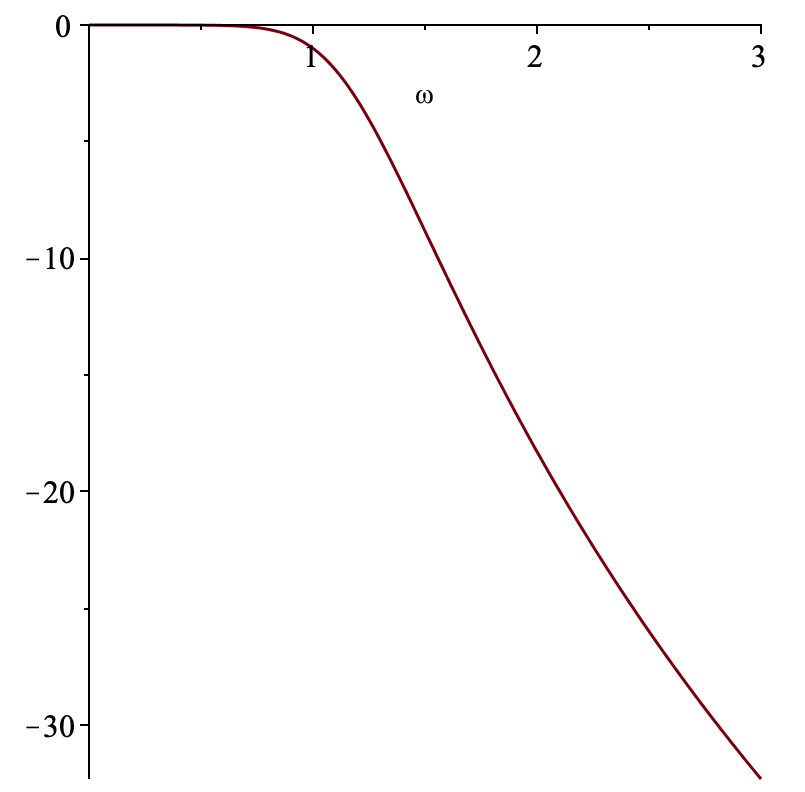
\includegraphics[scale=0.45]{maple3.png}
\caption{Modulová frekvenční charakteristika NDP - LC příčkový filtr}
\end{figure}
\noindent Hodnota přenosové funkce v 1 byla vyhodnocena jako $-1$.\\
\noindent Byla provedena transformace hodnot prvků normované dolní propusti (NDP) na~pásmovou propust (PP). Zakončovací rezistor byl zvolen 1\,$\Omega$, další dva parametry funkce značí spodní a horní hranici propustného pásma.\\
Prvky v první větvi obvodu byly vyčísleny jako $C_1 = 2.198$e-7\,F, $L1 = 5.144$e-6\,H, v druhé větvi $C_2 = 1.242$e-5\,F, $L_2 = 9.106$e-8\,H. Pro třetí větev $C_3 = 9.106$e-8\,F, $L_3 = 1.242$e-5\,H a pro čtvrtou $C_4 = 5.144$e-6\,F, $L_4 = 2.198$e-7\,H.\\
\noindent Vygenerovaná struktura je popsána na obrázku \ref{s:SCHEM1}.\\
\\
\begin{figure}[h]
\centering
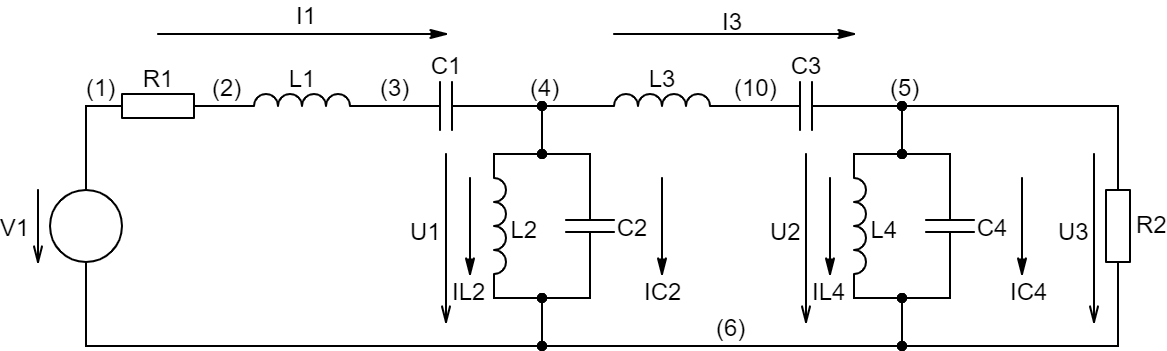
\includegraphics[scale=0.3]{Circuit(4).png}
\caption{Schéma LC příčkové struktury \label{s:SCHEM1}}
\end{figure}
\noindent Byly nastaveny jakosti cívek v LC příčkové struktuře na konečnou hodnotu. Funkce $MakeRealL$ zařadí do výsledné LC příčkové struktury sériově rezistory k induktorům podle zadaného činitele jakosti $Q$ a zadaného kmitočtu (ten odpovídá u pásmové propusti geometrickému středu propustného pásma --- nebo je možno zadat obě hranice propustného pásma). Byl zvolen činitel jakosti 100. Činitel jakosti je dán převrácenou hodnotou poměrné šířky pásma
\begin{equation}
Q = \frac{1}{B} = \frac{\omega_s}{\delta \omega},
\end{equation}
kde B je poměrná šířka pásma, $\delta \omega = \omega_2 - \omega_1$ a $\omega_s = \sqrt{\omega_1\omega_2}$. $\omega_1$ a $\omega_2$ zde jsou mezní kruhové kmitočty odpovídající poklesu přenosu filtru o 3\,dB.\\
\\
Pro kmitočtové pásmo stovky kHz až jednotky MHz v závislosti na typu jádra a kvalitě materiálu lze dosahovat hodnoty činitele jakosti cca 1000 a hodnoty indukčnosti řádově 100\,$\upmu$H až 10\,mH. Pro činitel jakosti se zde uplatňuje kmitočtová závislost $Q = \omega L/R$. Pro kmitočtové pásmo do 10\,kHz hodnoty činitele jakosti klesají řádově na hodnoty 10 pro velké hodnoty L. Výpočet sériového odporu je proveden podle předpisu $R_s~=~L1~\cdot~2~\pi~f/Q$. Pro první větev je $R_{s1} = 4.836$e-2\,$\Omega$, pro druhou $R_{s2} = 8.563$e-4\,$\Omega$, pro třetí $R_{s3} = 1.168$e-1\,$\Omega$ a $R_{s4} = 2.067$e-3\,$\Omega$.\\
\\
\noindent Byl spočten přenos pro LC strukturu bez a s přidanými sériovými rezistory. Pro oba přenosy byla vykreslena modulová frekvenční charakteristika. Přenosové funkce zde pro svou složitost a zachování přehlednosti textu nejsou uváděny, ale jsou k nalezení v přiloženém Maple skriptu.
\begin{figure}[h]
\centering
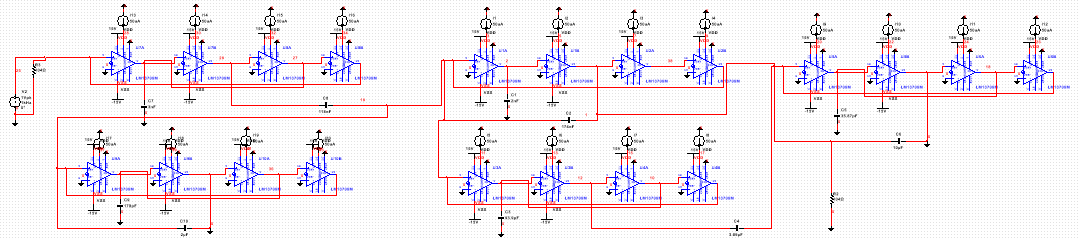
\includegraphics[scale=0.55]{maple4.png}
\caption[Modulová frekvenční charakteristika LC struktury a LC struktury s konečnou hodnotou jakostí cívek]{Modulová frekvenční charakteristika LC struktury (červená) a LC struktury s konečnou hodnotou jakostí cívek (zelená)}
\end{figure}
\begin{figure}[h]
\centering
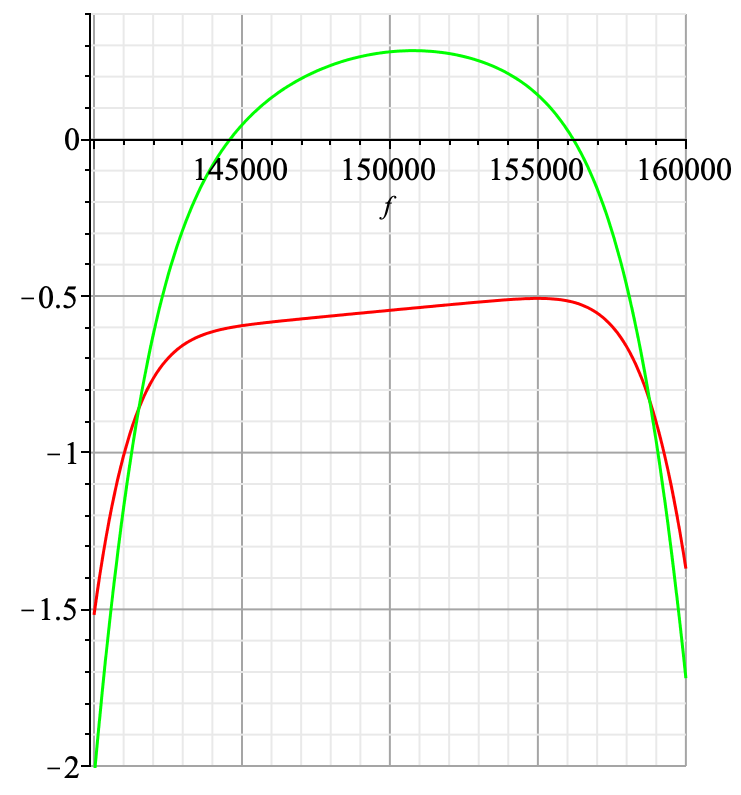
\includegraphics[scale=0.55]{maple5.png}
\caption[Přiblížená modulová frekvenční charakteristika LC struktury a LC struktury s konečnou hodnotou jakostí cívek]{Přiblížená modulová frekvenční charakteristika LC struktury (červená) a LC struktury s konečnou hodnotou jakostí cívek (zelená)}
\end{figure}
\noindent Vyčíslením v $f_m \cdot 2 \pi$ Hz, kde $f_m$ je geometrický střed propustného pásma, bylo obdrženo zesílení 1.052\,dB.\\
\\
\subsection{Simulace prvků LC prototypu}\label{s:ARC123}
V této sekci byl náhradou induktorů v LC prototypu za gyrátory obdržen návrh ARC filtru.\\
Zatím neodnormované prvky byly vyčísleny jako $C_1 = 2.198$e-7\,F, $C_2 = 1.242$e-5\,F, $C_3 = 9.106$e-8\,F, $C_4 = 5.144$e-6\,F, $L_1 = 5.144$e-6\,H, $L_2 = 9.106$e-8\,H, $L_3 = 1.242$e-5\,H, $L_4 = 2.198$e-7\,H, $R_1 = 1$\,$\Omega$, $R_z = 1$\,$\Omega$.\\
\\
\noindent Odnormované hodnoty kapacit získané vydělením kmitočtem $fp \cdot 2 \pi$, kde $fp$ je horní hranice propustného pásma, byly spočteny jako $C_1 = 2.187$e-13\,F, $C_2 = 1.235$e-11\,F, $C_3 = 9.058$e-14\,F, $C_4 = 5.117$e-12\,F.\\
\noindent Frekvenčně a impedančně odnormované odpory byly vypočteny podělením kmitočtem $fp \cdot 2 \pi$ a přibližnou hodnotou kapacity pro mikroelektronickou realizaci $C = 2$\,pF. Výsledné hodnoty jsou $R_1 = R_z = 497.359$\,k$\Omega$.\\
\noindent Využitím poznatků ze sekce \ref{s:GYR} byly dosazením do vztahu $C = L \cdot g_m^2$ s uvažováním minimální transkonduktance z datasheetu LM13700 ($g_m$ = 9600\,$\upmu$S) získány kapacity $C_{L1} = 4.741$e-10\,F, $C_{L2} = 8.392$e-12\,F, $C_{L3} = 1.145$e-9\,F, $C_{L4} = 2.026$e-11\,F.\\
\\
\noindent Výsledné hodnoty všech součástek s přesností na dvě desetinná místa jsou\\ $C1 = 21.87$\,pF, $C2 = 123.53$\,nF, $C3 = 905.75$\,pF, $C4 = 5.12$\,pF, $C_{L1} = 47.41$\,nF, $C_{L2} = 8.39$\,pF, $C_{L3} = 1.15$\,nF, $C_{L4} = 202.59$\,nF, $R1 = Rz = 497.36$\,k$\Omega$.
\subsection{Funkční simulace LC prototypu}\label{s:KASK2}
\noindent Základní myšlenka funkční simulace LC prototypu vychází z popisu příčkové struktury grafem signálových toků a simulací tohoto grafu vhodným elektronickým obvodem. Z~aproximace bylo kaskádní syntézou získáno rozložení výsledné přenosové funkce filtru na funkce jednotlivých kaskádně řazených bloků. Kaskádně spojené dvojbrany se~vzájemně neovlivňují --- v napěťovém módu mají charakter napětím řízených zdrojů napětí a v~proudovém módu proudem řízených zdrojů proudu. Přenos celé kaskády je dán součinem přenosů jednotlivých bloků. Na jeho základě se realizuje návrh filtru jako návrh jednotlivých bloků. Návrh je proveden s bloky s~jedním OTA a po realizaci lze jednotlivé bloky modifikovat jak z hlediska struktury, tak z hlediska hodnot jednotlivých prvků vybrané struktury. Například změnou transkonduktance jednotlivých bloků pak lze variabilně modifikovat mezní kmitočet.\\
\newpage
\noindent Analýzou LC struktury z Maplu byly obdrženy obvodové rovnice, kde R~je~volitelný~(fiktivní)~rezistor.
\begin{align}
I_1 &= \frac{1}{R_1 + pL_1 + \frac{1}{pC_1}}(U_G - U_1)\\
v_1 & = \frac{R}{R_1 + pL_1 + \frac{1}{pC_1}}(U_G - U_1)\\
U_1 &= \frac{1}{\frac{1}{pL_2} + pC_2}(I_1 - I_{3})\\
U_1 &= \frac{1}{\frac{R}{pL_2} + RpC_2}(v_1 - v_{3})\\
I_{3} &= \frac{1}{pL_3 + \frac{1}{pC_3}}(U_1 - U_2)\\
v_{3} &= \frac{R}{pL_3 + \frac{1}{pC_3}}(U_2 - U_3)\\
U_3 &= U_2 = \frac{1}{\frac{1}{R_z}+pC_4 + \frac{1}{pL_4}}(I_1 - I_{L2} - pC_2U_2)\\
U_3 &= U_2 = \frac{1}{\frac{R}{R_z}+RpC_4 + \frac{R}{pL_4}}(v_1 - U_2 - RpC_2 U_2)
\end{align}
\noindent To odpovídá realizační struktuře se čtyřmi bloky o přenosech $H_1, \ldots,H_4$.
\begin{align}
H_1 & = \frac{R}{R_1 + pL_1 + \frac{1}{pC_1}}\\
H_2 &= \frac{1}{\frac{R}{pL_2} + RpC_2}\\
H_3 &= \frac{R}{pL_3 + \frac{1}{pC_3}}\\
H_4 &= \frac{1}{\frac{R}{R_z}+RpC_4 + \frac{R}{pL_4}}
\end{align}
\subsection{Simulace obvodu}
\noindent  Zapojení s OTA vychází z již uvedených principů v sekci \ref{s:NAH}. K simulaci byly použity vypočtené hodnoty ze sekce \ref{s:ARC123}. \\
\\
\noindent Bylo použito zapojení se vstupním odporem $R_0$ řazeným paralelně ke zdroji (vhodnější pro funkční simulaci - Schaumann, Valkenburg \cite{13} str. 639) a nahrazení odporů bloky OTA. Šířka propustného pásma byla pro klidový stejnosměrný pracovní proud $I_{ABC} = 50$\,$\upmu$A odečtena jako 26.3\,kHz (obrázek \ref{s:BUT11} a \ref{s:BUT12}). Geometrický střed propustného pásma odpovídá 125.42\,kHz. Přeladěním filtru změnou klidového stejnosměrného pracovního proudu na $I_{ABC} = 100$\,$\upmu$A byla obdržena šířka propustného pásma 21.66\,kHz a geometrický střed propustného pásma 250.75\,kHz (obrázek \ref{s:BUT31} a \ref{s:BUT32}). \\
\\
Pro obdržení geometrického středu propustného pásma $f_m = 150$\,kHz je třeba zvolit klidový stejnosměrný pracovní proud $I_{ABC} = 59.82$\,$\upmu$A (obrázek \ref{s:BUT21} a \ref{s:BUT22}). Byla odečtena šířka propustného pásma 50.72\,kHz a útlum v propustném pásmu 56\,dB. \\
Pro obdržení geometrického středu propustného pásma $f_m = 100$\,kHz je třeba zvolit klidový stejnosměrný pracovní proud $I_{ABC} = 39.89$\,$\upmu$A. Byla odečtena šířka propustného pásma 20.18\,kHz a útlum v propustném pásmu 53.7--56.7\,dB (obrázek \ref{s:BUT01} a \ref{s:BUT02}).\\
\\
Analýzou obvodu s hodnotami komponent z Maplu bylo obdrženo bylo určeno THD a šum. Byl použit klidový stejnosměrný pracovní proud $I_{ABC} = 39.89$\,$\upmu$A odpovídající geometrickému středu propustného pásma 100~kHz. Šum zde byl počítán jako výkon signálu ve zvoleném uzlu vydělený celkovým výkonem tepelného šumu na standardní teplotě (27\,$^{\circ}$C). Je to tedy poměr vstupního SNR k~výstupnímu SNR. Jak lze vidět z tabulky \ref{s:THD111}, odstup signál šum je nejmenší pro frekvenci 100\,kHz odpovídající geometrickému středu propustného pásma.
\begin{table}[h]
\centering
  \begin{tabular}{ | c | c | c |}
    \hline
     Frekvence [kHz] & Odečtený šum [dB] \\ \hline
    1 & 121.201 \\ \hline
    10 & 100.583 \\ \hline
    100 & 53.665 \\ \hline
    1000 & 108.486 \\ \hline
  \end{tabular}
  \caption[Šum pro PP 4. řádu (Maple)]{Šum pro PP 4. řádu s výsledky z Maplu \label{s:THD111}}
\end{table}
\noindent Také bylo změřeno THD se základní frekvenci 100\,kHz, viz tabulka \ref{s:THD333}. Dle očekávání je nejnižší pro nejmenší počet harmonických frekvencí.
\begin{table}[h]
\centering
\renewcommand{\arraystretch}{1.15}
  \begin{tabular}{ | c | c | c |}
    \hline
    Frekvence zdroje [kHz] & Počet harmonických frekvencí & THD [\%] \\ \hline
	\multirow{3}{*}{100} & 3 & 2.161\\& 5 & 2.946 \\& 10 & 3.222 \\ \hline
  \end{tabular}
  \caption[THD pro PP 4. řádu (Maple)]{THD pro PP 4. řádu s výsledky z Maplu \label{s:THD333}}
\end{table}